\begin{frame}{$W(G)$ պարամետրի գնահատականներ}{մուլտիգրաֆների համար}

Եթե $G \in \mathfrak{N}$ և
\begin{itemize}
\item $G$-ն եռանկյուն չպարունակող գրաֆ է, ապա $W(G)\leq \vert V(G)\vert -1$ (Հասրաթյան, Քամալյան, 1987)
\item $|V(G)|\geq 2$, ապա\\ $W(G)\leq 2|V(G)|-3$ (Քամալյան, 1990)
\item $|V(G)|\geq 3$, ապա\\ $W(G)\leq 2|V(G)|-4$ (Գիառո և այլոք, 2001)
\end{itemize}

Պետրոսյանը (2010) ցույց է տվել, որ $2$ գործակիցը ընդհանուր դեպքում հնարավոր չէ լավացնել:

\end{frame}

\begin{frame}{$W(G)$ պարամետրի գնահատականներ}{հարթ գրաֆների համար}
 
\begin{theorem}[Աքսենովիչ, 2002]
Եթե $G$-ն կապակցված հարթ գրաֆ է և $G \in \mathfrak{N}$, ապա 
\begin{center}
$W(G) \leq \frac{11}{6}|V(G)|$:
\end{center}
\end{theorem}

\pause
\begin{hypothesis}[Աքսենովիչ, 2002]
Եթե $G$-ն կապակցված հարթ գրաֆ է և $G \in \mathfrak{N}$, ապա 
\begin{center}
$W(G) \leq \frac{3}{2}|V(G)|$:
\end{center}
\end{hypothesis}
\end{frame}

\begin{frame}[shrink]{$W(G)$ պարամետրի գնահատականներ}{մուլտիգրաֆների համար}
\begin{theorem}[1.2.8]
Եթե $G$-ն $2$-կապակցված մուլտիգրաֆ է և $G\in \mathfrak{N}$, ապա
\begin{center}
$W(G)\leq 1+\left\lfloor \frac{c(G)}{2}\right\rfloor(\Delta(G)-1)$,
\end{center}
որտեղ $c(G)$-ն $G$-ի ամենամեծ պարզ ցիկլի երկարությունն է:
\end{theorem}

\begin{hide}
\begin{corollary}
\label{c1_upper_V/2} Եթե $G$-ն $2$-կապակցված մուլտիգրաֆ է և $G\in \mathfrak{N}$, ապա
\begin{center}
$W(G)\leq 1+\left\lfloor \frac{\vert
V(G)\vert}{2}\right\rfloor(\Delta(G)-1)$:
\end{center}
\end{corollary}
% \end{frame}

% \begin{frame}{$W(G)$ պարամետրի գնահատականներ}{փոքր առավելագույն աստիճան ունեցող մուլտիգրաֆների համար}
\begin{corollary}
\label{c1_upper_Delta4} Եթե $G$-ն $2$-կապակցված մուլտիգրաֆ է,
$\Delta(G)\leq 4$ և $G\in \mathfrak{N}$, ապա
$W(G)\leq 3\left\lfloor \frac{\vert V(G)\vert}{2}\right\rfloor+1$:
\end{corollary}
% \pause
\end{hide}

\begin{corollary}[1.2.11]
Եթե $G$-ն $2$-կապակցված հարթ գրաֆ է, ընդ որում
$\Delta(G)\leq 4$ և $G\in \mathfrak{N}$, ապա 
$W(G)\leq \frac{3}{2}\vert V(G)\vert$:
\end{corollary}

Վերջին հետևանքը հաստատում է Աքսենովիչի հիպոթեզը միջակայքային ներկելի $2$-կապակցված հարթ գրաֆների համար, որոնց առավելագույն աստիճանը չի գերազանցում $4$-ը:
\end{frame}

\begin{frame}{$W(G)$ պարամետրի գնահատականներ}{համասեռ մուլտիգրաֆների համար}

\begin{corollary}[1.2.13]
Եթե $G$-ն կապակցված խորանարդ մուլտիգրաֆ է և $G\in \mathfrak{N}$, ապա
\begin{center}
$W(G)\leq \vert V(G)\vert+1$:
\end{center}
\end{corollary}

Ցույց է տրվել, որ այս վերին գնահատականները հասանելի են:

\begin{figure}[t!]
    \centering
    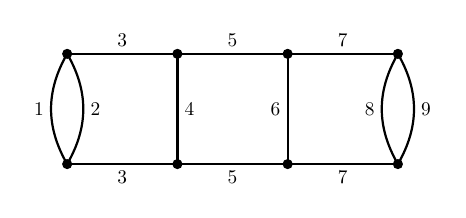
\begin{tikzpicture}[style=thick,scale=0.7, every node/.style={scale=0.7}]
        \coordinate (V11) at (2cm,2cm);
        \coordinate (V12) at (4cm,2cm);
        \coordinate (V13) at (6cm,2cm);
        \coordinate (V14) at (8cm,2cm);
        \coordinate (V21) at (2cm,4cm);
        \coordinate (V22) at (4cm,4cm);
        \coordinate (V23) at (6cm,4cm);
        \coordinate (V24) at (8cm,4cm);
        
        \draw (V11) -- node [below] {$3$} (V12) -- node [below] {$5$} (V13) -- node [below] {$7$} (V14);
        \draw (V21) -- node [above] {$3$} (V22) -- node [above] {$5$} (V23) -- node [above] {$7$} (V24);
        
        \draw (V11) edge [bend left] node [left] {$1$} (V21);
        \draw (V11) edge [bend right] node [right] {$2$} (V21);
        \draw (V12) -- node[right] {$4$} (V22);
        \draw (V13) -- node[left] {$6$} (V23);
        \draw (V14) edge [bend left] node [left] {$8$} (V24);
        \draw (V14) edge [bend right] node [right] {$9$} (V24);
        
        \draw[fill=black] (V11) circle (2pt) ;
        \draw[fill=black] (V12) circle (2pt) ;
        \draw[fill=black] (V13) circle (2pt) ;
        \draw[fill=black] (V14) circle (2pt) ;
        \draw[fill=black] (V21) circle (2pt) ;
        \draw[fill=black] (V22) circle (2pt) ;
        \draw[fill=black] (V23) circle (2pt) ;
        \draw[fill=black] (V24) circle (2pt) ;
    \end{tikzpicture}
    \end{figure}

\begin{hide}
\begin{theorem}
\label{t1_upper_bounds_are_sharp} Ցանկացած $n,r\geq 2$ ամբողջ թվերի համար գոյություն ունի $2$-կապակցված $G$ մուլտիգրաֆ, որի համար $\vert V(G)\vert =2n$ և
$\Delta(G)=r$, այնպես, որ $G\in \mathfrak{N}$ և $W(G)=1+n(r-1)$:
\end{theorem}
\end{hide}
\end{frame}

\begin{frame}{$w(G)$ պարամետրի գնահատականներ}
\begin{theorem}[1.2.15]
Եթե $G$-ն կապակցված մուլտիգրաֆ է և $G\in \mathfrak{N}$, ապա
\begin{center}
$w(G)\geq \left\lceil \frac{\vert V(G)\vert}{2\cdot
\alpha'(G)}\right\rceil\delta(G)$:
\end{center}
\end{theorem}
Այս թեորեմը ընդհանրացնում է Հանսոնի և Լոտենի կողմից $(a,a-1)$-երկհամասեռ երկկողմանի գրաֆների համար ստացված արդյունքը:

\pause

\begin{figure}[h]
\begin{center}
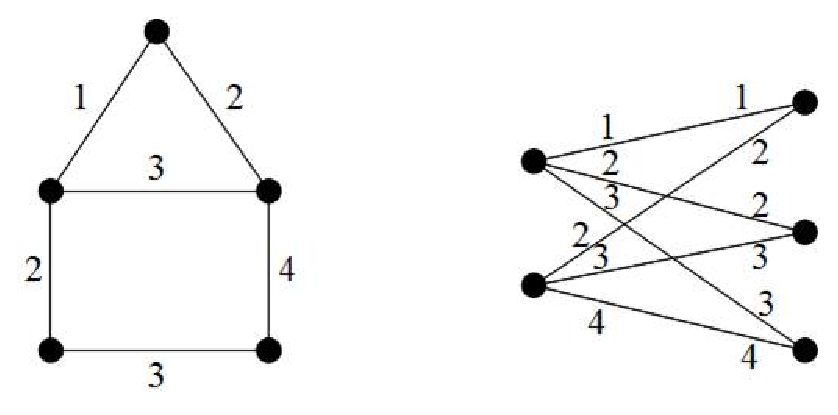
\includegraphics[width=0.5\textwidth]{figures/W-bound-fig1.eps}
\end{center}
\end{figure}
\end{frame}


\begin{frame}{$w(G)$ պարամետրի գնահատականներ}
\begin{corollary}[1.2.16]
Եթե $G$ կապակցված մուլտիգրաֆը չունի կատարյալ զուգակցում և $G\in \mathfrak{N}$, ապա
\begin{center}
$w(G)\geq \max\{\Delta(G),2\delta(G)\}$:
\end{center}
\end{corollary}

\pause

\begin{theorem}[1.2.17]
Եթե $G$-ն կապակցված կենտ մուլտիգրաֆ է, $\vert
E(G)\vert-\frac{\vert V(G)\vert}{2}$ թիվը կենտ է և $G\in \mathfrak{N}$,
ապա
\begin{center}
$w(G)\geq \max\{\Delta(G),2\delta(G)\}$:
\end{center}
\end{theorem}
\end{frame}


\begin{frame}{$w(G)$ պարամետրի գնահատականներ}{Օրինակ}
\begin{columns}
\begin{column}{0.45\textwidth}
\begin{itemize}
    \item $G$-ի բոլոր գագաթների աստիճանները կենտ են,
    \item $|E(G)|-\frac{|V(G)|}{2}=15$,
    \item $w(G) \geq 6$:
\end{itemize}
    
\end{column}
\begin{column}{0.55\textwidth}
\begin{figure}[h]
\begin{center}
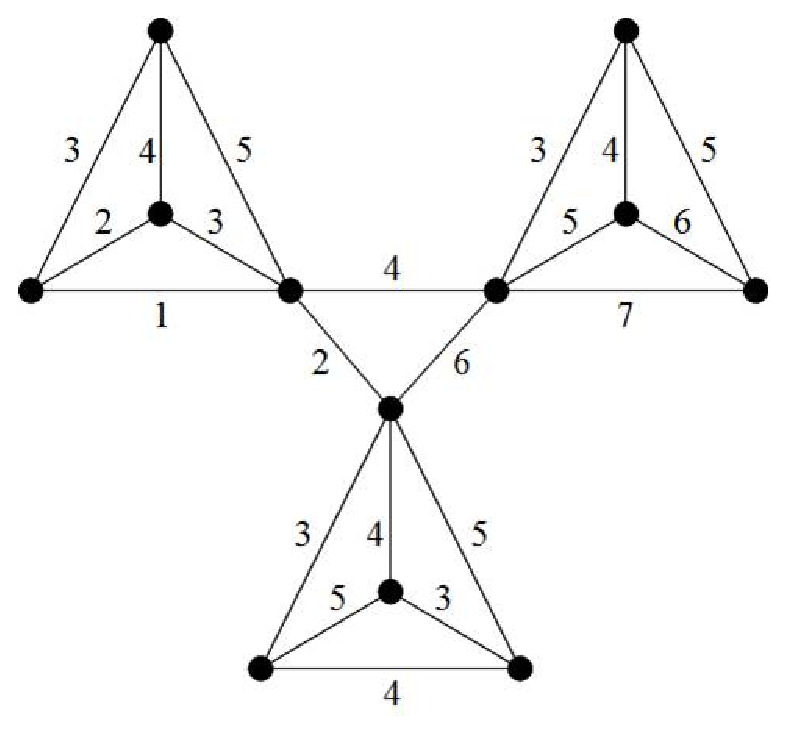
\includegraphics[width=\textwidth]{figures/W-bound-fig2.eps}
\end{center}
\end{figure}

\end{column}
\end{columns}
\end{frame}